\documentclass{article}
\setlength{\parindent}{0pt}
\usepackage[a4paper,margin=2.5cm]{geometry}
\usepackage{listings}

% External links
\usepackage{hyperref}

% Colored text
\usepackage{xcolor}
% Graphics
\usepackage{graphicx}

% Customized table
\usepackage{float}
\usepackage{array}
\newcolumntype{L}[1]{>{\raggedright\arraybackslash}p{#1}}
\usepackage{booktabs}

% Create plots
\usepackage{pgfplots}
\usepackage{pgf-pie}

\title{QS-Report für MS6}
\author{Syntax Syndicate - Casono}
\begin{document}
\maketitle

\section{Einleitung}
Dieses Dokument ist die Fortsetzung des QA-Konzeptes für unser Mehrspieler-Spiel \textit{Casono}.
Es wurde von uns als Teil der Programmierprojekt-Vorlesung (ehemals bekannt als cs108) an der Universität Basel von uns entwickelt.

Dieser Report folgt dem selben \textit{DIN ISO 9126}, und ist wie auch das Konzept für den ersten Teil in die selben Themenbereiche unterteilt:
\begin{itemize}
  \item \textbf{Konstruktives Qualitätsmanagement} - Maßnahmen, die \emph{während} der Entwicklung ergriffen werden, um die Qualität von Anfang an sicherzustellen.
  Einschließlich technischer Standards, Werkzeuge und internen Organisation.
  \item \textbf{Analytisches Qualitätsmanagement} - Maßnahmen zur \emph{Kontrolle und Untersuchung} des bestehenden Produkts, durch Anwendung automatisierte Analysen, Metrik-Schwellenwerte und Unit-Tests.
\end{itemize}

\section{Konstruktives Qualitätsmanagement}
Ein konstruktives Qualitätsmanagement umfasst alle Maßnahmen, die proaktiv Mängel verhindern, indem gemeinsame Standards, Prozesse und Werkzeuge festgelegt werden, die jedes Teammitglied während der Entwicklung einhält.

\subsection{Technische Maßnahmen}

\subsubsection{JavaDoc}
JavaDoc wurde genutzt um alle Öffentlichen Klassen, Interfaces, Records und Methoden zu dokumentieren.
Als Teil der GitLab-Build-Pipeline wird JavaDoc auf Richtigkeit überprüft. Werden strukturelle Fehler wie ungültige Referenzen erkannt, schlägt die Pipeline fehl und der Merge wird verhindert.\\

Unsere implizite Form für JavaDoc-Kommentare ist wie folgt:
\begin{itemize}
  \item Eine prägnante Zusammenfassung in einem Satz in der ersten Zeile
  \item Zusätzliche Informationen oder Beispiele in weiteren Absätzen.
  \item Dokumentation aller Parameter (\texttt{@param}), Rückgabewerte (\texttt{@return}) und Fehler (\texttt{@throws}).
\end{itemize}
Leider konnten wir das in MS4 vorgenommene Ziel, das auch Warnungen zu einem Abbruch der Pipeline führen, aus Technischen Gründen nicht umsetzen.

\newpage
\subsubsection{Logging}
Das Projekt verwendet Log4J~2 (\texttt{log4j-api} und \texttt{log4j-core} zur Laufzeit) zusammen mit Jansi für eine farbige Konsolenausgabe.
Das Format der Ausgabe ist durch eine Konfigurationsdatei vereinheitlicht.\\

Die Protokollstufen werden wie folgt einheitlich verwendet:
\begin{itemize}
  \item \texttt{DEBUG} für interne Zustandsänderungen
  \item \texttt{INFO} für Lebenszyklusereignisse wie Serverstart, Verbindungsaufbau/-trennung des Clients
  \item \texttt{WARN} für behebbare Anomalien
  \item \texttt{ERROR} für nicht behebbare Fehler
\end{itemize}

Im Gegensatz zu MS4 wurden die Namen der Logger gekürzt und nicht mehr der gesamte Classpath verwendet. Ein Beispiel für die Ausgabe sieht so aus:
\begin{figure}[H]
  \centering
  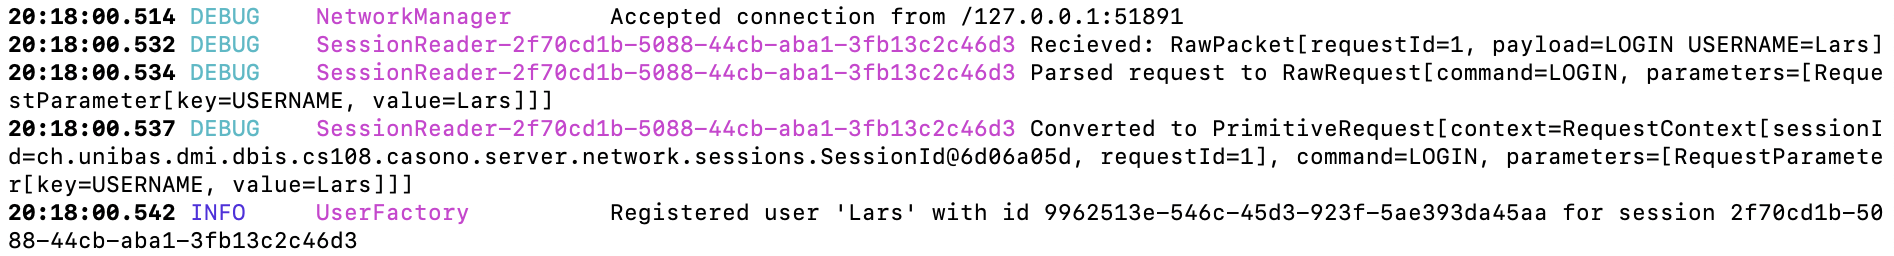
\includegraphics[width=\textwidth]{../../images/milestones/ms-6/qa-report/server_log.png}
  \caption{Konsolenausgabe des Servers während dem Verbindungsaufbau und Anmeldung eines Nutzers}
\end{figure}

\subsection{Organisatorische Maßnahmen}

\subsubsection{Teamkultur und die \texttt{CONTRIBUTORS}-Datei}
Das Stammverzeichnis des GitLab-Repositories enthält eine Datei namens \texttt{CONTRIBUTORS.md}, die die seit MS4 unveränderten Teamkonventionen dokumentiert:
\begin{itemize}
  \item Die Verwendung von Branches - Feature-Branches werden in \texttt{main} zusammengeführt
  \item Merge-Richtlinie - CI muss bestanden werden. Eine Genehmigung durch Kollegen ist wünschenswert wenn Änderungen an dessen Code vorgenommen wurden.
  \item Namenskonventionen für Branches und Commits
  \item Code-Stil - Google-Java-Format, AOSP-Variante, Einrückung mit vier Leerzeichen
  \item Jede Änderung beginnt mit einem Issue oder Task in GitLab, bevor mit der Umsetzung begonnen wird
  \item Branch-Namen folgen dem Muster \texttt{<typ>/<kurzbeschreibung>} gemäß \href{https://conventional-branch.github.io/}{Conventional Branch} Standard
  \item Commit-Messages folgen dem \href{https://www.conventionalcommits.org/en/v1.0.0/}{Conventional Commits} Standard
  \item Code-Style wird durch Linter (Checkstyle) und Formatter (Spotless, Google/AOSP Java Style) automatisiert überprüft
  \item Merge Anfragen müssen eine Beschreibung enthalten und auf das zugehörige Issue oder den Task verweisen
  \item Zusammenarbeit und Kommunikation erfolgen bevorzugt über Issue-Kommentare, nicht über private Nachrichten
\end{itemize}

\subsubsection{GitLab-Task- und Issue-Vorlagen für Fortschrittsverfolgung}
GitLab-Vorlagen für Tasks und Issues werden für alle geplanten Arbeitselemente verwendet. Die Aufgabenvorlage sorgt für eine einheitliche Struktur, die die Fortschrittsverfolgung erleichtert und das Risiko vager oder unvollständiger Arbeitselemente reduziert.

Durch die Vergabe von Labels kann Tasks und Issues weiterer Kontext gegeben werden.

\newpage
\section{Analytisches Qualitätsmanagement}

\subsection{Analytische Verfahren}

\subsubsection{Eigentumsrechte an Programmcode über GitLab \texttt{CODEOWNERS}}
In unserem Konzept haben wir uns vorgenommen, durch eine \texttt{CODEOWNERS} Datei den Teammitgliedern die Eigentumsrechte ihres Programmcodes zuzusprechen. Leider hat sich bestätigt das die von SciCORE betriebene Instanz nicht die Premium-Stufe hat, wodurch diese Funktion für uns nicht zur Verfügung steht. \\

Statt auf eine Automatisierte Grundlage zu vertrauen, haben wir uns für den nächstbesten Weg der Disziplinarität entschieden, wie am Beispiel von \href{https://git.scicore.unibas.ch/cs108-fs26/Gruppe-13/-/merge_requests/166}{dieser Merge-Anfrage} gesehen werden kann.

\subsubsection{Automatisiertes CI-Linting und Build-Verifizierung}
Jeder Push und jede Merge-Anfrage löst die CI-Pipeline aus.

Für Pushes und Merge-Anfragen setzt sich die Pipeline aus folgenden Phasen zusammen:
\begin{enumerate}
  \item \textbf{Linting-Phase} \textcolor{blue}{[Push, MR]} - Checkstyle und Spotless überprüfen, ob der Programmcode dem vereinbarten Stil entspricht.
  \item \textbf{Build-Phase} \textcolor{blue}{[Push, MR]} - \texttt{./gradlew assemble} prüft, ob das gesamte Projekt fehlerfrei kompiliert werden kann.
  \item \textbf{Checkstyle-Report} \textcolor{blue}{[MR]} - Ein zusätzlicher Checkstyle-Report wird für Merge-Anfragen erzeugt und als Code-Quality-Report bereitgestellt.
  \item \textbf{Javadoc-Prüfung} \textcolor{blue}{[MR]} - JavaDoc wird auf Korrektheit geprüft.
  \item \textbf{Test-Phase} \textcolor{blue}{[Push, MR]} - Automatisierte Tests werden ausgeführt und ein Testreport erzeugt.
\end{enumerate}
Die Entscheidung das fehlgeschlagene Jobs keinen Push aber dafür eine Merge-Anfrage verhindern können, hat sich als vernünftig bewehrt.
Über die Dauer des Projektes hat diese Pipeline mehrmals verhindert das Fehlerhafter oder sogar kaputter Programmcode in den main Branch gelangen konnte.

\newpage
\subsection{Testverfahren}
Unit-Tests wurden mit \textit{JUnit 5} geschrieben und in der Testphase der CI-Pipeline ausgeführt. Ein fehlgeschlagener Test blockiert die Merge-Anfrage.

Als weiteres Werkzeug verwendeten wir \textit{JaCoCo} für die Ermittlung der Testabdeckung. \\
Die Testabdeckung für Meilenstein sechs ist wie folgt:

\begin{table}[H]
  \centering
  \renewcommand{\arraystretch}{1.4}
  \begin{tabular}{L{7.5cm} r r}
    \textbf{Paketname (gekürzt)}        & \textbf{Instr.\ Cov.} & \textbf{Branch Cov.} \\
    \midrule
    \texttt{client.chat}                                & 30\,\%  & 16\,\% \\
    \texttt{client.game}                                & 15\,\%  & 2\,\% \\
    \texttt{client.network}                             & 2\,\%  & 1\,\% \\
    \texttt{client.ui} (von Abdeckung ausgeschlossen)   & 0\,\%  & 0\,\% \\
    \texttt{server.app.checks}                          & 0\,\%  & 0\,\% \\
    \texttt{server.app.commands}                        & 0\,\%  & 0\,\% \\
    \texttt{server.domain.game}                         & 68\,\%  & 43\,\% \\
    \texttt{server.domain.*}                            & 59\,\%  & 44\,\% \\
    \texttt{server.network.transport}                   & 0\,\%  & 0\,\% \\
    \texttt{server.network.protocol}                    & 67\,\%  & 55\,\% \\
    \texttt{server.network.*}                           & 67\,\%  & 55\,\% \\
    \midrule
    \textbf{Summe}                          & \textbf{18\,\%} & \textbf{11\,\%} \\
    \bottomrule
  \end{tabular}
\end{table}

Im vierten Meilenstein haben wir uns das Ziel gesetzt die Testabdeckung für die Game-Engine und wichtige Netzwerkkomponenten auf mindestens 50\% zu erhöhen, dieses Ziel haben wir laut JaCoCo nicht erreicht.\\
Geht man jedoch nach der Abdeckung der "Test Runner for Java" Erweiterung in VSCode, dann beträgt die Abdeckung 51\%. Sowohl Julian (Game-Engine) als auch Lars (Serverseitiges Netzwerk) haben sich nach diesen Angaben gereichtet, weshalb wir dachten wir hätten unser Ziel erreicht.

\begin{figure}[H]
  \centering
  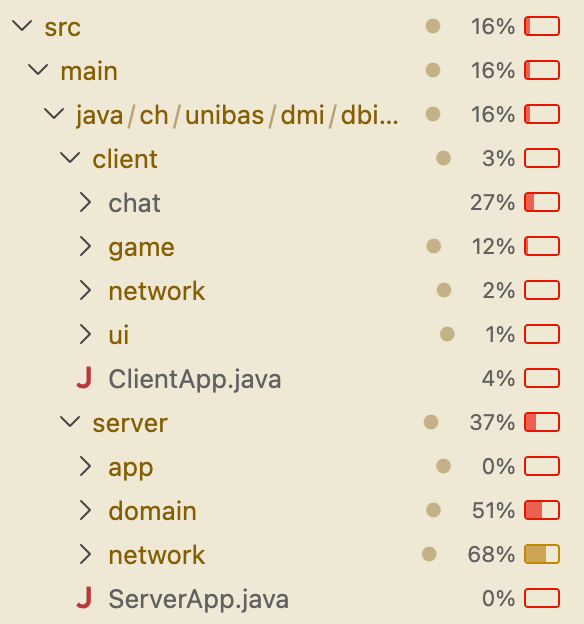
\includegraphics[width=0.4\textwidth]{../../images/milestones/ms-6/qa-report/vscode_code_coverage.png}
  \caption{Abweichende Angaben bezüglich der Abdeckung von VSCode zu JaCoCo}
\end{figure}

Die Verwendung zwei unterschiedlicher Tools zur Beurteilung des Fortschritts ist definitiv etwas, was es in Zukunft zu vermeiden gilt.

\newpage
\section{Metriken}
\textit{Die nachfolgenden Metriken wurden am 17. Mai 2026 um 20:58 Uhr erhoben, neuere Änderungen sind daher nicht berücksichtigt.}

\subsection{Lines of Code}
\begin{figure}[H]
  \centering
  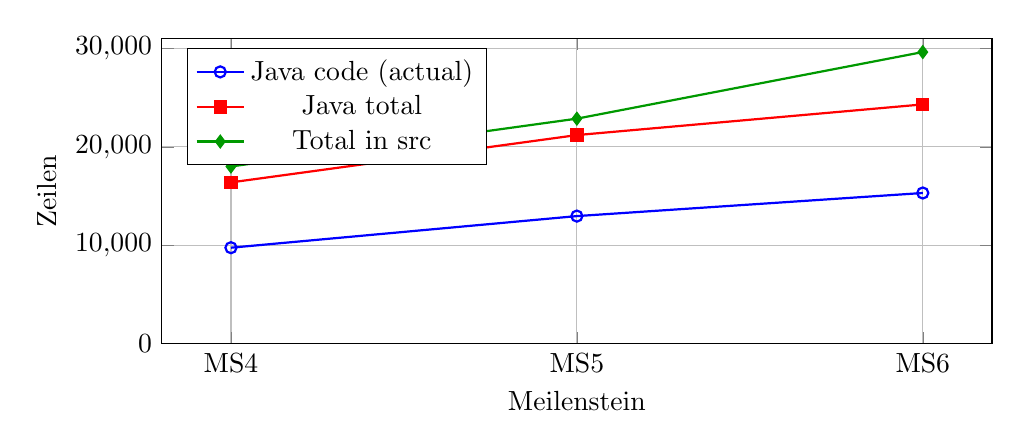
\begin{tikzpicture}
  \begin{axis}[
    width=\textwidth,
    height=0.45\textwidth,
    xlabel={Meilenstein},
    ylabel={Zeilen},
    ymin=0,
    ymax=31000,
    xtick={1,2,3},
    xticklabels={MS4,MS5,MS6},
    legend pos=north west,
    grid=both,
    scaled y ticks=false,
    yticklabel style={/pgf/number format/fixed}
  ]

  % Actual Java code
  \addplot[
    color=blue,
    mark=o,
    thick
  ]
  coordinates {
    (1,9760)
    (2,12972)
    (3,15319)
    };
  \addlegendentry{Java code (actual)}

  % Total Java
  \addplot[
    color=red,
    mark=square*,
    thick
  ] 
  coordinates {
    (1,16396)
    (2,21203)
    (3,24319)
  };
  \addlegendentry{Java total}

  % Total in src
  \addplot[
    color=green!60!black,
    mark=diamond*,
    thick
  ] 
  coordinates {
    (1,18012)
    (2,22872)
    (3,29639)
  };
  \addlegendentry{Total in src}

  \end{axis}
  \end{tikzpicture}
  \caption{Entwicklung der Java-Zeilen (tatsächlicher Code vs. Gesamt) über die Meilensteine hinweg}
\end{figure}

\subsection{Verteilung der Code-Zeilen auf verschiedene Dateitypen}
\begin{figure}[H]
  \centering
  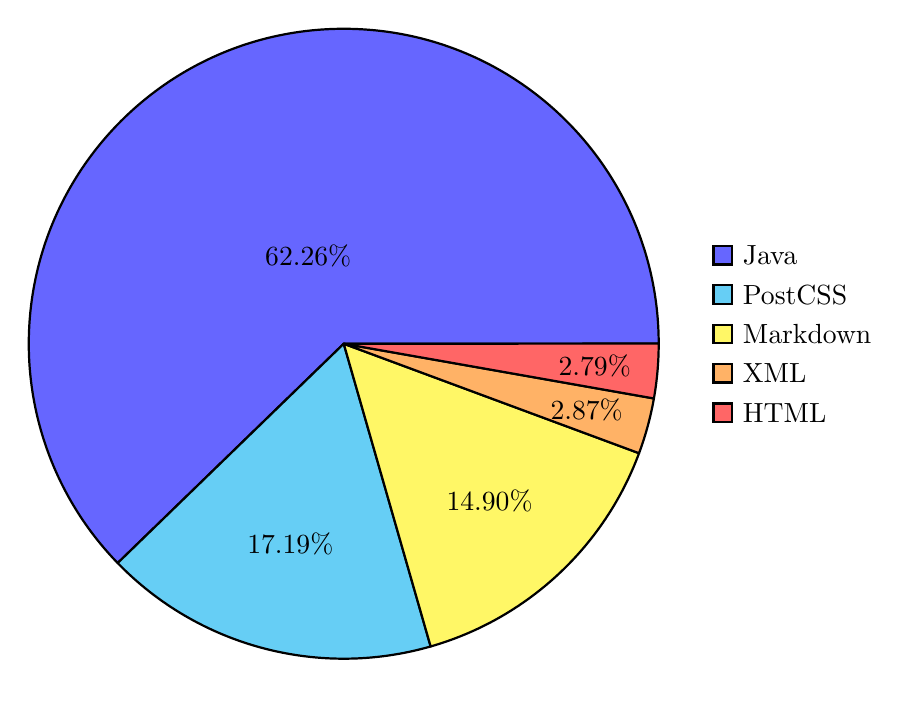
\begin{tikzpicture}
    \pie[
      text=legend,
      radius=4
    ]{
      62.26/Java,
      17.19/PostCSS,
      14.90/Markdown,
      2.87/XML,
      2.79/HTML
    }
  \end{tikzpicture}
  \caption{Verteilung der Code-Zeilen (Top 5 Dateitypen)}
  \label{fig:loc-pie}
\end{figure}

\end{document}
